\documentclass[12pt, trans]{beamer}


\mode<presentation>{
	\usetheme{Copenhagen}
	
	\usecolortheme[RGB={0, 0, 102}]{structure}
	  % or ...
	
	  %\setbeamercovered{transparent}
	  % or whatever (possibly just delete it)
	  
	%\usecolortheme{albatross}
	%\usecolortheme{lily}
	
	\useinnertheme{rectangles}
	\useoutertheme{smoothbars}
	\usefonttheme{structurebold}
}

\definecolor{HuskyPurple}{RGB}{57, 39, 91}
\definecolor{HuskyGold}{RGB}{226, 210, 163}
\definecolor{CalBlue}{RGB}{0, 0, 102}
\definecolor{CalGold}{RGB}{255, 204, 51}

%\beamertemplateshadingbackground{HuskyPurple}{CalBlue}

%\beamersetaveragebackground{HuskyPurple}

%\beamertemplateballitem

%turn off never-used navigation symbols: 
\setbeamertemplate{navigation symbols}{}


\usepackage{MnSymbol}

%%% Page Number
\setbeamertemplate{footline}[page number] 


%%%%%%

\usepackage[english]{babel}
% or whatever

%\usepackage[latin1]{inputenc}

\def\name{Christine Kuang, Siqi Wu, and Angie Zhu}
\hypersetup{
  %colorlinks = true,
  urlcolor = black,
  pdfauthor = {\name},
  pdfkeywords = {},
  pdftitle = {},
  pdfsubject = {},
  pdfpagemode = UseNone
}



\newcommand{\mypurple}{\color{HuskyPurple}}
\newcommand{\mygold}{\color{CalGold}}
%\newcommand{\sascode}{\ttfamily \color{magenta}}

% ==========================================================


%% for displaying Chinese
\usepackage{fontspec,xltxtra,xunicode}
\usepackage[slantfont,boldfont]{xeCJK}

% 设置中文字体
% ==========================================================
\setCJKmainfont[BoldFont=STHeiti]{STSong}
\setCJKsansfont{STHeiti}
\setCJKmonofont{STFangsong}
 
\setCJKfamilyfont{zhsong}{STSong}
\setCJKfamilyfont{zhhei}{STHeiti}
\setCJKfamilyfont{zhfs}{STFangsong}
\setCJKfamilyfont{zhkai}{STKaiti}
 
\newcommand*{\songti}{\CJKfamily{zhsong}} % 宋体
\newcommand*{\heiti}{\CJKfamily{zhhei}}   % 黑体
\newcommand*{\kaishu}{\CJKfamily{zhkai}}  % 楷书
\newcommand*{\fangsong}{\CJKfamily{zhfs}} % 仿宋
% ==========================================================

%%%%%%%%%%
% the following are user defined commands

\newcommand{\pr}[1]{{\mathbb P}\left(#1\right)}        % probability
\newcommand{\E}[1]{{\mathbb E}\left[#1\right]}        % expectation 
\newcommand{\1}[1]{{\mathbf 1}\left\{#1\right\}}        % indicator
\newcommand{\V}[1]{\text{Var}\left(#1\right)}    % variance

\def\lp{\left(}
\def\rp{\right)}


%%%%%%%%%%%%%%%%%%%%%%%%%%%%%%
%%%%%%%%%%%%%%%%%%%%%%%%%%%%%%

\title{Sina Weibo as a Corpus for Studying Public Opinions}
\author[Kuang, Wu, and Zhu]{\name}
\institute{Department of Statistics, UC Berkeley}
\date{May 3, 2012}

%\pgfdeclareimage[width=0.35in]{logo}{piggy.jpg}
%\logo{\pgfuseimage{logo}}

\begin{document}



\frame{\titlepage}

%%%%
\begin{frame}
\frametitle{Outline}
\tableofcontents%[pausesections]
\end{frame}


%%%%%%%%%%%%%%%
\section{Introduction}

\begin{frame}{Introduction}

\note{


Due to the restriction on overseas websites such as Facebook or Twitter, domestic substitutes have become the major platforms for the internet citizens to express their opinions towards various social or political issues. Studying posts on those website thus provides interesting insights into the public opinion. For example, some events in the recent years, such as the tragic Wenzhou train collision on July 23 2011
%\footnote{For details, see \url{http://en.wikipedia.org/wiki/Wenzhou_train_collision}. }
  and the more recent Wang Lijun incident,
%\footnote{For details, see \url{http://en.wikipedia.org/wiki/Wang_Lijun_incident}.}  
have split the public into two major groups among which one considers the government's way of dealing with those incidences is good and one does not. 
In principle, we can draw text data from those websites identifying whether a particular post is related to the event of interest, and which group the post should be classified into.

Sina Weibo 新浪微博 is the largest microblogging website and one of the most popular social network website in China. It had more than 300 million registered users as of February 2012 
%(\cite{bloombergSina})
and accounted for 65\% of China's microblog market by pageviews as of December 2011
%(\cite{WashingtonPostSina}).
In this project, we develop a framework for for studying public opinions using Sina Weibo as a corpus for a given topic. Posts are sampled from Weibo and then processed taking the characteristics of both Chinese language and Weibo posts into consideration.

Analysis part...
}

\begin{itemize}[<+->]
\item Opinions on microblogging and social networking websites
\item Sina Weibo 新浪微博 is the largest microblogging website: \\
	 accounted for 65\% of China's microblog market as of December 2011
\item Study public opinions using Sina Weibo as a corpus for a given topic
\end{itemize}

\end{frame}


%%%%%%%%%%%%%%%
\begin{frame}{Topic}

\note{
Internet has been heavily censored in China. In order to collect representative samples, political topics are off the table. 
Also the samples will be time sensitive.

2012-04-16, 17

Due to the restrictions on API we will discuss in a few slides, ``hot'' topics are preferred.

}

\begin{itemize}[<+->]
\item Internet censorship in China
\item Time sensitive
\item Processing is topic-dependent
\item Hot topic is preferred %due to API restriction
\item Chosen topic: Han Han 韩寒
\end{itemize}

\end{frame}



%%%%%%%%%%%%%%%
\begin{frame}{Background}

\note{
%\footnote{ {\em Han Han: China's Literary Bad Boy} by Simon Elegant Monday, Nov. 02, 2009, Time Magazine, \url{http://www.time.com/time/magazine/article/0,9171,1931619,00.html}. }
}

 \begin{columns}[t]
 \begin{column}{0.6\textwidth}

	\begin{itemize}[<+->]
	\item  HAN Han 韩寒 (born 23 September 1982) is a Chinese best-selling author, professional rally driver, and  wildly  popular blogger
	\item Published his first novel {\em Triple Gate 三重门} at age of 17
	\item High school dropout
	\end{itemize}

 \end{column}
 
 \begin{column}{0.45\textwidth}
	\begin{figure}
	  \centering
	  \includegraphics[scale=0.4]{han_han.jpg} 
	\end{figure}

{\tiny Photograph by Tony Law / Redux. Source: \url{http://www.time.com/time/magazine/article/0,9171,1931619,00.html}}
 \end{column}
 
 \end{columns}

\end{frame}



%%%%%%%%%%%%%%%
\begin{frame}{Background}

\begin{itemize}[<+->]
\item Ghostwriting allegation against Han from January 2012
\item FANG Zhouzi 方舟子, a scientific author and anti-fraud crusader, created widespread debate on the internet
\item 光明与磊落
\item Han received a death threat on April 15, 2012
\end{itemize}

\end{frame}


%%%%%%%%%%%%%%%%
%%\section{Data}

\begin{frame}{Data Collection}
\note{


Sina Weipo provides an application programming interface (API) to access their public data.


Some technical issues: how do we access data from those website? We now have implemented a python crawler, but i believe there is a upperbound for the data you can collect within a fixed amount of time due to the weibo restriction. 
How do we design our sampling scheme? we want a way to sample data such that they can represent the whole user group of weibo. we need to know the behavior of the weibo users as some of them simply have nothing to do and posting junks all days. stratified sampling based on province? 
}

\begin{itemize}[<+->]
\item Topic searching via API: \\only the latest results are returned\\up to 30 each time
\item Collected on April 16 and 17, 2012
\end{itemize}

\end{frame}



%%%%%%%%%%%%%%%%%%%%%%%%%%%%%%%
%%%%%%%%%%%%%%%%%%%%%%%%%%%%%%%

\section{Processing}
%%%%%%

\begin{frame}{Characteristics of Chinese Language}

\begin{itemize}[<+->]
\item No explicit delimiter
\item Ambiguities in phrases
	\begin{itemize}
	\item Context ambiguition: e.g., 他好吃
	\item Word definition ambiguition: e.g., 打
	\end{itemize}
\item Out-of-vocabulary words
\item No 1-to-1 correspondence between traditional and simplified Chinese
\end{itemize}

\end{frame}


%%%%%%%%%%%%%%%%
\begin{frame}{Characteristics of Sina Weibo Posts}

\note{
A post can be text, an image, video, or other multimedia.

}

\begin{itemize}[<+->]
\item  .
\end{itemize}

\end{frame}

%%%%%%%%%%%%%%%
\begin{frame}{Pre-tagging Processing}

\begin{itemize}[<+->]
\item  .
\end{itemize}

\end{frame}


%%%%%%%%%%%%%%%%
\begin{frame}{Tagging}

\begin{itemize}[<+->]
\item  Process: tagged 3000 total posts with four categories
\item Examples:
	\begin{description}
	\item[Positive] 支持韩寒! Support Han Han!
	\item[Negative] 看到韩寒就恶心。 Feel nauseous when I see Han Han.
	\end{description}


\item Limitations:
	
	\begin{itemize}
	\item Subjective responses:\\
		\quad e.g., ``that wasn't too bad''
	\item 	Uncertain tags
		\begin{itemize}
		\item Quotes
		\item Posts without subjects
		\item Posts that just mention opposing author
		\end{itemize}
	\end{itemize}

\end{itemize}

\end{frame}

%%%%%%%%%%%%%%%
\begin{frame}{Pre-segmentation Processing}

\begin{itemize}[<+->]
\item .
\end{itemize}

\end{frame}


%%%%%%%%%%%%%%%%
\begin{frame}{Segmentation}

\begin{itemize}[<+->]
\item  .
\end{itemize}

\end{frame}

%%%%%%%%%%%%%%%
\begin{frame}{Conjunction Rules}

\begin{itemize}[<+->]
\item  .
\end{itemize}

\end{frame}

%%%%%%%%%%%%%%%
\begin{frame}{Stop Words and Punctuation Elimination}

\begin{itemize}[<+->]
\item .
\end{itemize}

\end{frame}



%%%%%%%%%%%%%%%%%%%%%%%%%%%%%%%
%%%%%%%%%%%%%%%%%%%%%%%%%%%%%%%
\section{EDA}

%%%%%%%%%%%%%%%
\begin{frame}{EDA}

\begin{itemize}[<+->]
\item $\geq 10$
\end{itemize}

\end{frame}



%%%%%%%%%%%%%%%
\begin{frame}{Word frequency}
\begin{itemize}[<+->]
\item Extract the word frequency vector $x_i$ from the $i$-th post
\item Construct the word frequency matrix $X=(x_1,...,x_n)^T$. This will be our design matrix.
\end{itemize}
\end{frame}
%%%%%%%%%%%%%%%%%%%%


\begin{frame}{Word frequency visualization: matrix plot}

\begin{figure}
  \centering
  \includegraphics[height=0.9\textheight]{./../../wordFreqMat.png} 
\end{figure}


\end{frame}

%%%%%%%%%%%%%%%
\begin{frame}{Co-occurrance}

\begin{figure}
  \centering
  \includegraphics[height=0.9\textheight]{./../../coocurResults/cooccurMatPlot.png} 
\end{figure}


\end{frame}

%%%%%%%%%%%%%%%
\begin{frame}{Co-occurrance}

\begin{figure}
  \centering
  \includegraphics[height=0.9\textheight]{./../../coocurResults/cooccurNetwork.png} 
\end{figure}

\end{frame}

%%%%%%%%%%%%%%%
\begin{frame}[fragile]{Sparse graphical models}

\begin{itemize}[<+->]
\item Fact: if $x\in R^p$ follows $N(\mu,\Sigma)$, then for $i\ne j$
\begin{align*}
(x_i  \upmodels % mnsymbol
x_j )\mid \{x_{\text{all but $(i,j)$}}\} \textbf{ iff } (\Sigma^{-1})_{ij}=0
\end{align*}
\item This motivates us to estimate $\Sigma^{-1}$.
\item Let $x_1,x_2,...x_n$ be IID $N(\nu,\Sigma)$ data. The joint likelihood of the data is
\begin{align*}
& f(x_1, \dots, x_n|\mu,\Sigma) 
\\&= \frac{1}{(2\pi \det\lp \Sigma\rp)^{n/2}}\exp\left\{ -\frac{1}{2} \sum_{i=1}^n(x_i-\mu)^T\Sigma^{-1}(x_i-\mu) \right\}.
\end{align*}

\end{itemize}

\end{frame}


%%%%%%%%%%%%%%%%
\begin{frame}[fragile]{Sparse graphical models (cont'd)}

\begin{itemize}[<+->]
\item  Log-likelihood:
\begin{align*}
l(\mu,\Sigma^{-1}) = -\frac{n}{2}\log \det \lp \Sigma \rp  -\frac{1}{2} \sum_{i=1}^n(x_i-\mu)^T\Sigma^{-1}(x_i-\mu)
\end{align*}

\item Do a maximum likelihood estimation (optimize over $\mu$ and $S = \Sigma^{-1}$; easy to see that the MLE for $\mu$ is $\bar{x}$):

\begin{align*}
\max_S\left\{  \frac{n}{2}\log \det\lp S \rp  -\frac{1}{2} \sum_{i=1}^n(x_i-\bar{x})^T S (x_i-\bar{x})\right\} 
\end{align*}


\end{itemize}

\end{frame}

%%%%%%%%%%%%%%%
\begin{frame}[fragile]{Sparse graphical models (cont'd)}

\begin{itemize}[<+->]
\item  Here comes the trace trick $\sum_{i=1}^n(x_i-\mu)^T S (x_i-\mu) = \textbf{Tr} (\sum_{i=1}^n (x_i-\mu)(x_i-\mu)^TS) = n\textbf{Tr}(\hat{\Sigma}S)$. We end up with the optimization problem for fitting a Gaussian graphical model:

\begin{align*}
\max_S \left\{  \log \det \lp S\rp - \textbf{Tr}\lp \hat{\Sigma}S \rp  \right\}
\end{align*}

\item  Fitting a sparse Gaussian graphical model:
\begin{align*}
\max_S \left\{ \log \det S - \textbf{Tr} \lp \hat{\Sigma}S \rp - \lambda ||S||_1 \right\}
\end{align*}
where $||S||_1 = \sum_{i,j}|s_{ij}|$. See, e.g. Banerjee et al. (2007) and Friedman et al. (2007). 

\end{itemize}

\end{frame}

%%%%%%%%%%%%%%%%
\begin{frame}{Sparse graphical models: results}

\begin{figure}
  \centering
  \includegraphics[height=0.9\textheight]{./../../gLassoResults/glasso1.png} 
\end{figure}

\end{frame}

%%%%%%%%%%%%%%%
\begin{frame}{Sparse graphical models: results}

\begin{figure}
  \centering
  \includegraphics[height=0.9\textheight]{./../../gLassoResults/glasso2.png} 
\end{figure}

\end{frame}
%%%%%%%%%%%%%%%
\begin{frame}{Sparse graphical models: results}

\begin{figure}
  \centering
  \includegraphics[height=0.9\textheight]{./../../gLassoResults/glasso3.png} 
\end{figure}

\end{frame}
%%%%%%%%%%%%%%%
\begin{frame}{Sparse graphical models: results}

\begin{figure}
  \centering
  \includegraphics[height=0.9\textheight]{./../../gLassoResults/glasso4.png} 
\end{figure}

\end{frame}
%%%%%%%%%%%%%%%
\begin{frame}{Sparse graphical models: results}

\begin{figure}
  \centering
  \includegraphics[height=0.9\textheight]{./../../gLassoResults/glasso5.png} 
\end{figure}

\end{frame}
%%%%%%%%%%%%%%%
\begin{frame}{Sparse graphical models: results}

\begin{figure}
  \centering
  \includegraphics[height=0.9\textheight]{./../../gLassoResults/glasso6.png} 
\end{figure}

\end{frame}

%%%%%%%%%%%%%%%%
\begin{frame}{Sparse graphical models v.s. co-occurence}

 \begin{columns}[t]
 \begin{column}{0.5\textwidth}

\begin{figure}
  \centering
  \includegraphics[scale=0.25]{./../../gLassoResults/glasso1.png} 
\end{figure}

 \end{column}
 \begin{column}{0.5\textwidth}

\begin{figure}
  \centering
  \includegraphics[scale=0.25]{./../../coocurResults/cooccurNetwork.png} 
\end{figure}

 \end{column}
 \end{columns}

\end{frame}

\clearpage 
%%%%%%%%%%%%%%%%%%%%%%%%%%%%%%
%%%%%%%%%%%%%%%%%%%%%%%%%%%%%%
\section{Classification}

\begin{frame}{Classification}

\note{ I will talk about this slide and Christine continues the next}

\begin{itemize}[<+->]


\item $x_i\in R^{p}$ be the $i$-th row of $X\in R^{3000\times795}$
\item $y_i$ the corresponding category. Assume $y_i\in\{-1,+1\}$, where the $+1$ can have the following meanings:
  \begin{itemize}[<+->]
    \item positive opinion towards Han Han; 
    \item negative opinion towards Han Han; 
    \item netural or unidentifiable opinion; 
    \item spam. 
\end{itemize}
\item Two classification methods: LASSO and $l_1$-norm SVM.
\end{itemize}
\end{frame}
%%%%%%%%%%%%%%%
\subsection{LASSO}

%%%
\begin{frame}[fragile]{LASSO}
\begin{itemize}[<+->]

\item The Lasso approach (Tibshirani, (1996)):
\[
\hat{\beta}(\lambda) = \arg \min_\beta \frac{1}{2}||y-(\beta_0+X\beta)||_2^2 + \lambda ||\beta||_1
\]
\item The classifier:
\[
\text{class}(x) = \textbf{sign}(\beta_0+x^T\beta)\in\{-1,+1\}
\]

\item Four models for each category for classification
\item General overview of method
\item General overview of application to data
	\begin{itemize}
	\item for 4 categories
	\item 10 fold CV
	\item Frequency matrix is $3000 \times 795$
	\item classification error
	\end{itemize}
	
\end{itemize}

\end{frame}

%%%%%%%%%%%%%%%%
\begin{frame}{Choosing $\lambda$: cross-validation}

\begin{figure}
  \centering
  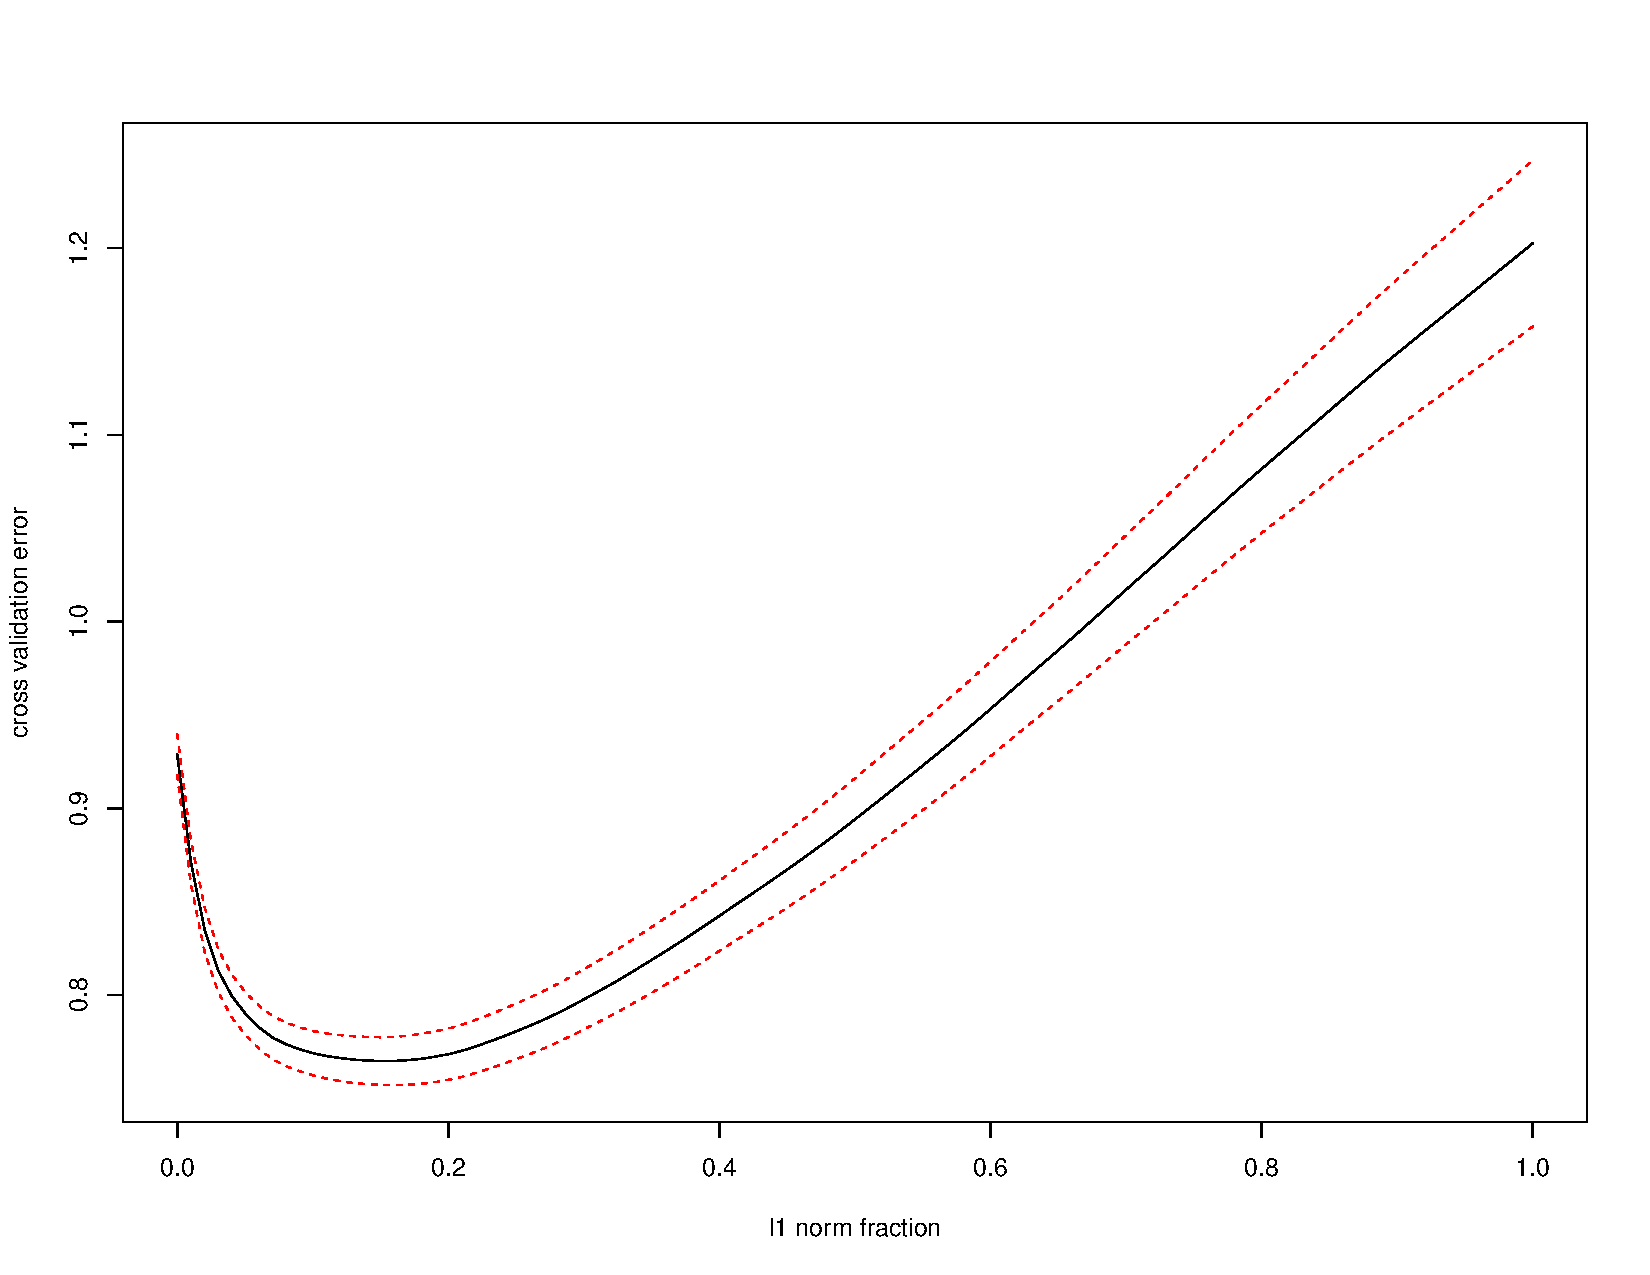
\includegraphics[height=0.9\textheight]{./../../lassoResults/CVPosErr.pdf} 
\end{figure}

\end{frame}


%%%
\begin{frame}{LASSO Results} 

\begin{itemize}[<+->]
\item Three different ways to look at coefficients
\item Why: can look at the classifier:
\[
\text{class}(x) = \textbf{sign}(\beta_0+x^T\beta)\in\{-1,+1\}
\]
	\begin{itemize}
	\item Absolute value: most relevant/predictive words
	\item Positive: more likely to classify the post in +1 category (all other covariates being fixed)
	\item Negative: less likely to be in -1 category	
	\end{itemize}
	
\end{itemize}

\end{frame}



%%%%%%%%%%%%%%%
\begin{frame}{Positive v.s. Nonpositive classification result}

\begin{itemize}[<+->]
\item +1: positive opinion;
\item -1: non-positive opinion, including negative, neutral and spam.
\end{itemize}

\tiny
\begin{center}
\begin{tabular}{|c|c||c|c||c|c|}
\hline
Word & Absolute Coef. & Word & Positive Coef. & Word & Negative Coef.\\ \hline \hline
加油 & 0.820 & 加油 & 0.820 & 样子 & -0.396\\
(keep going) & & (keep going) & & (manner) & \\\hline
韩少 & 0.644 & 韩少 & 0.644 & 恋 & -0.344\\
(Master Han) & & (Master Han) & & (love) & \\\hline
成熟 & 0.546 & 成熟 & 0.546 & 发表 & -0.336\\
(mature) & & (mature) & & (announce) & \\\hline
顶 & 0.533 & 顶 & 0.533 & 道理 & -0.336\\
(support) & & (support) & & (rational) & \\\hline
宽容 & 0.518 & 宽容 & 0.518 & 利益 & -0.335\\
(tolerant) & & (tolerant) & & (benefit) & \\\hline
\end{tabular}
LASSO word images for the positive v.s. nonpositive classification.
\end{center}


\end{frame}


%%%%%%%%%%%%%%%%
\begin{frame}{Negative v.s. Nonnegative classification result}
\note{
(To Angie: please delete the zero entries)
(To Christine: remember to talk about why there are four empty entries; this is probably due to the size of nega sample is too small)
}
\begin{itemize}[<+->]
\item +1: negative opinion;
\item -1: non-negative opinion, including positive, neutral and spam.
\end{itemize}

\tiny
\begin{center}
\begin{tabular}{|c|c||c|c||c|c|}
\hline
Word & Absolute Coef. & Word & Positive Coef. & Word & Negative Coef.\\ \hline \hline
讨厌 & 0.481 & 讨厌 & 0.481 & 支持 & -0.008\\
(hate) & & (hate) & & (support) & \\\hline
无耻 & 0.412 & 无耻 & 0.412 & 不 & 0.000\\
(shameless) & & (shameless) & & (no) & \\\hline
恶心 & 0.395 & 恶心 & 0.395 & 人 & 0.000\\
(disgusting) & & (disgusting) & & (people/person) & \\\hline
骗子 & 0.380 & 骗子 & 0.380 & 说 & 0.000\\
(liar) & & (liar) & & (say) & \\\hline
扁 & 0.353 & 扁 & 0.353 & 方舟子 & 0.000\\
(beat up) & & (beat up) & & (FangZhouZi) & \\\hline
\end{tabular}
LASSO word images for the negative v.s. negative classification.
\end{center}

\end{frame}


%%%%%%%%%%%%%%%%
%%\begin{frame}{LASSO: Negative}
%%
%%\begin{figure}
%%  \centering
%%  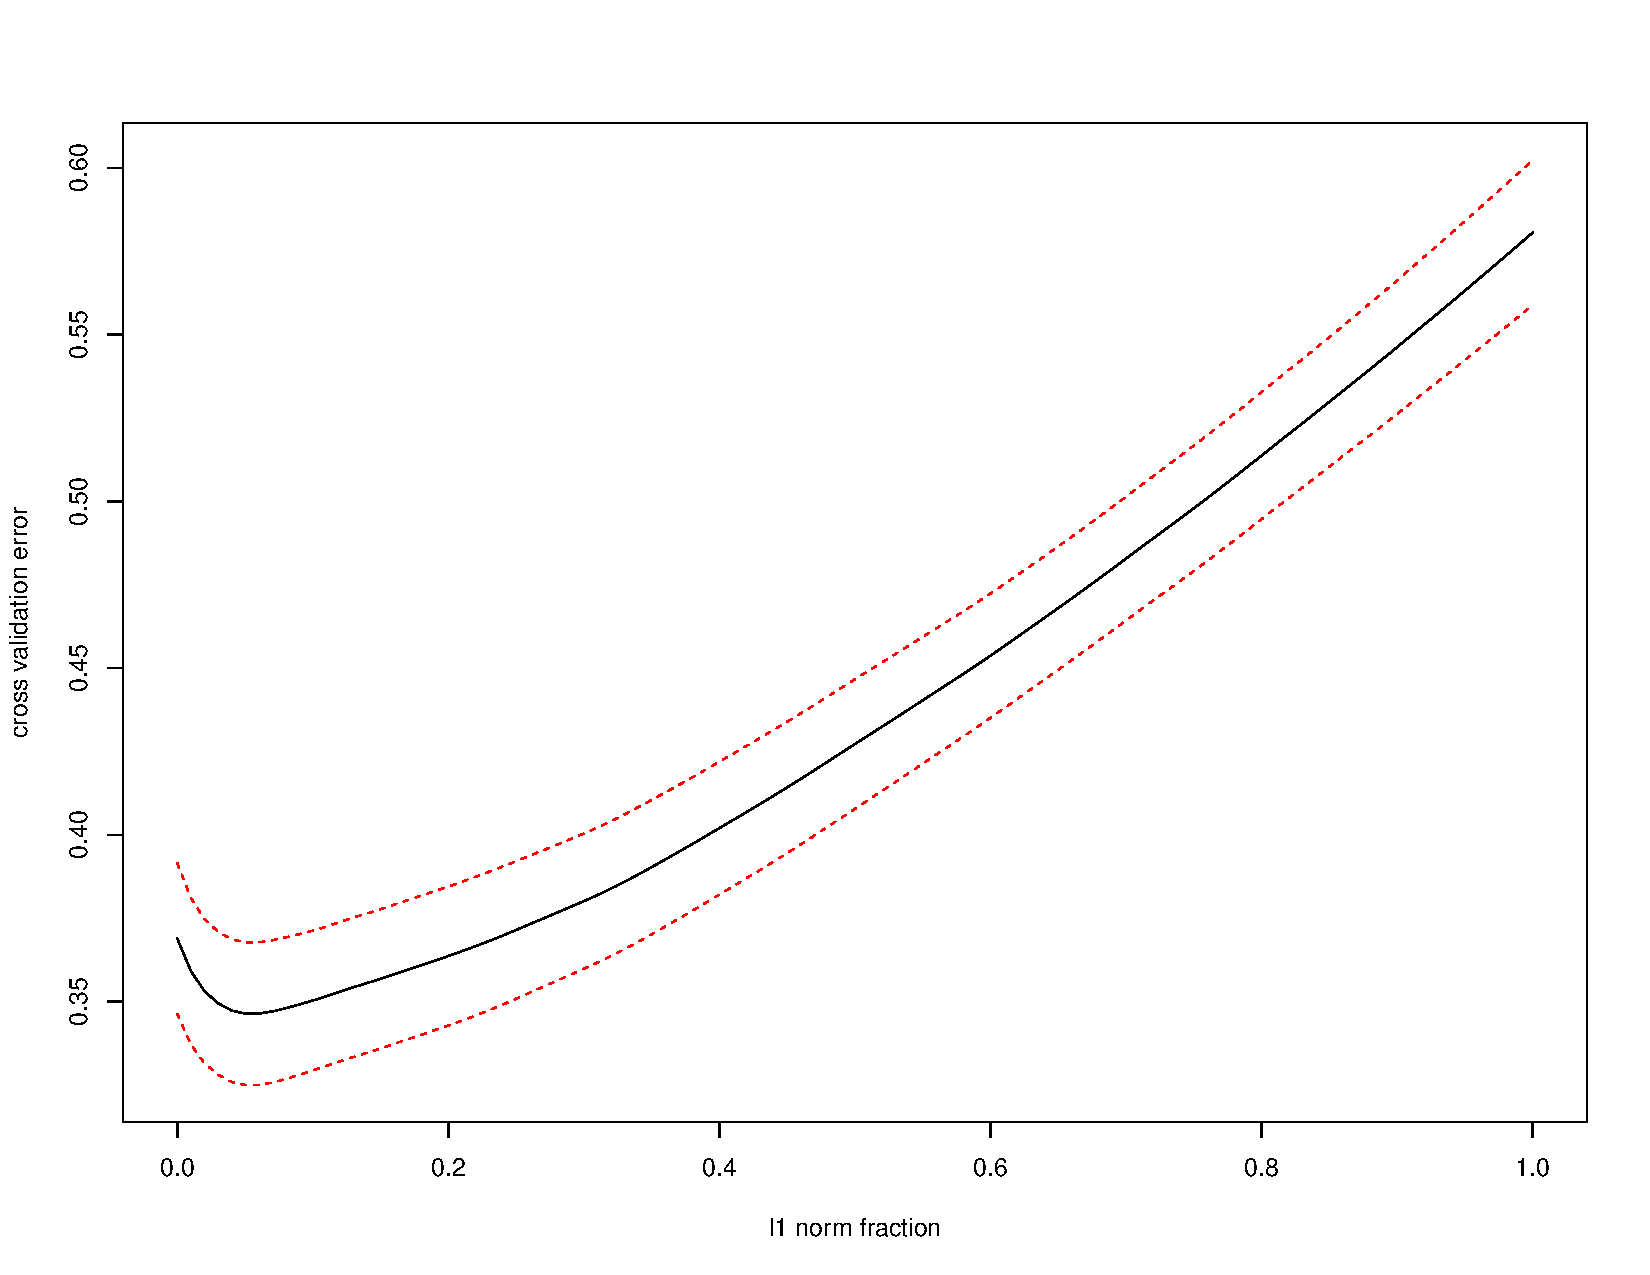
\includegraphics[height=0.9\textheight]{./../../lassoResults/CVNegErr.pdf} 
%%\end{figure}
%%
%%\end{frame}
%%
%%%%%%%%%%%%%%%%%
%%\begin{frame}{LASSO: Neutral}
%%
%%\begin{figure}
%%  \centering
%%  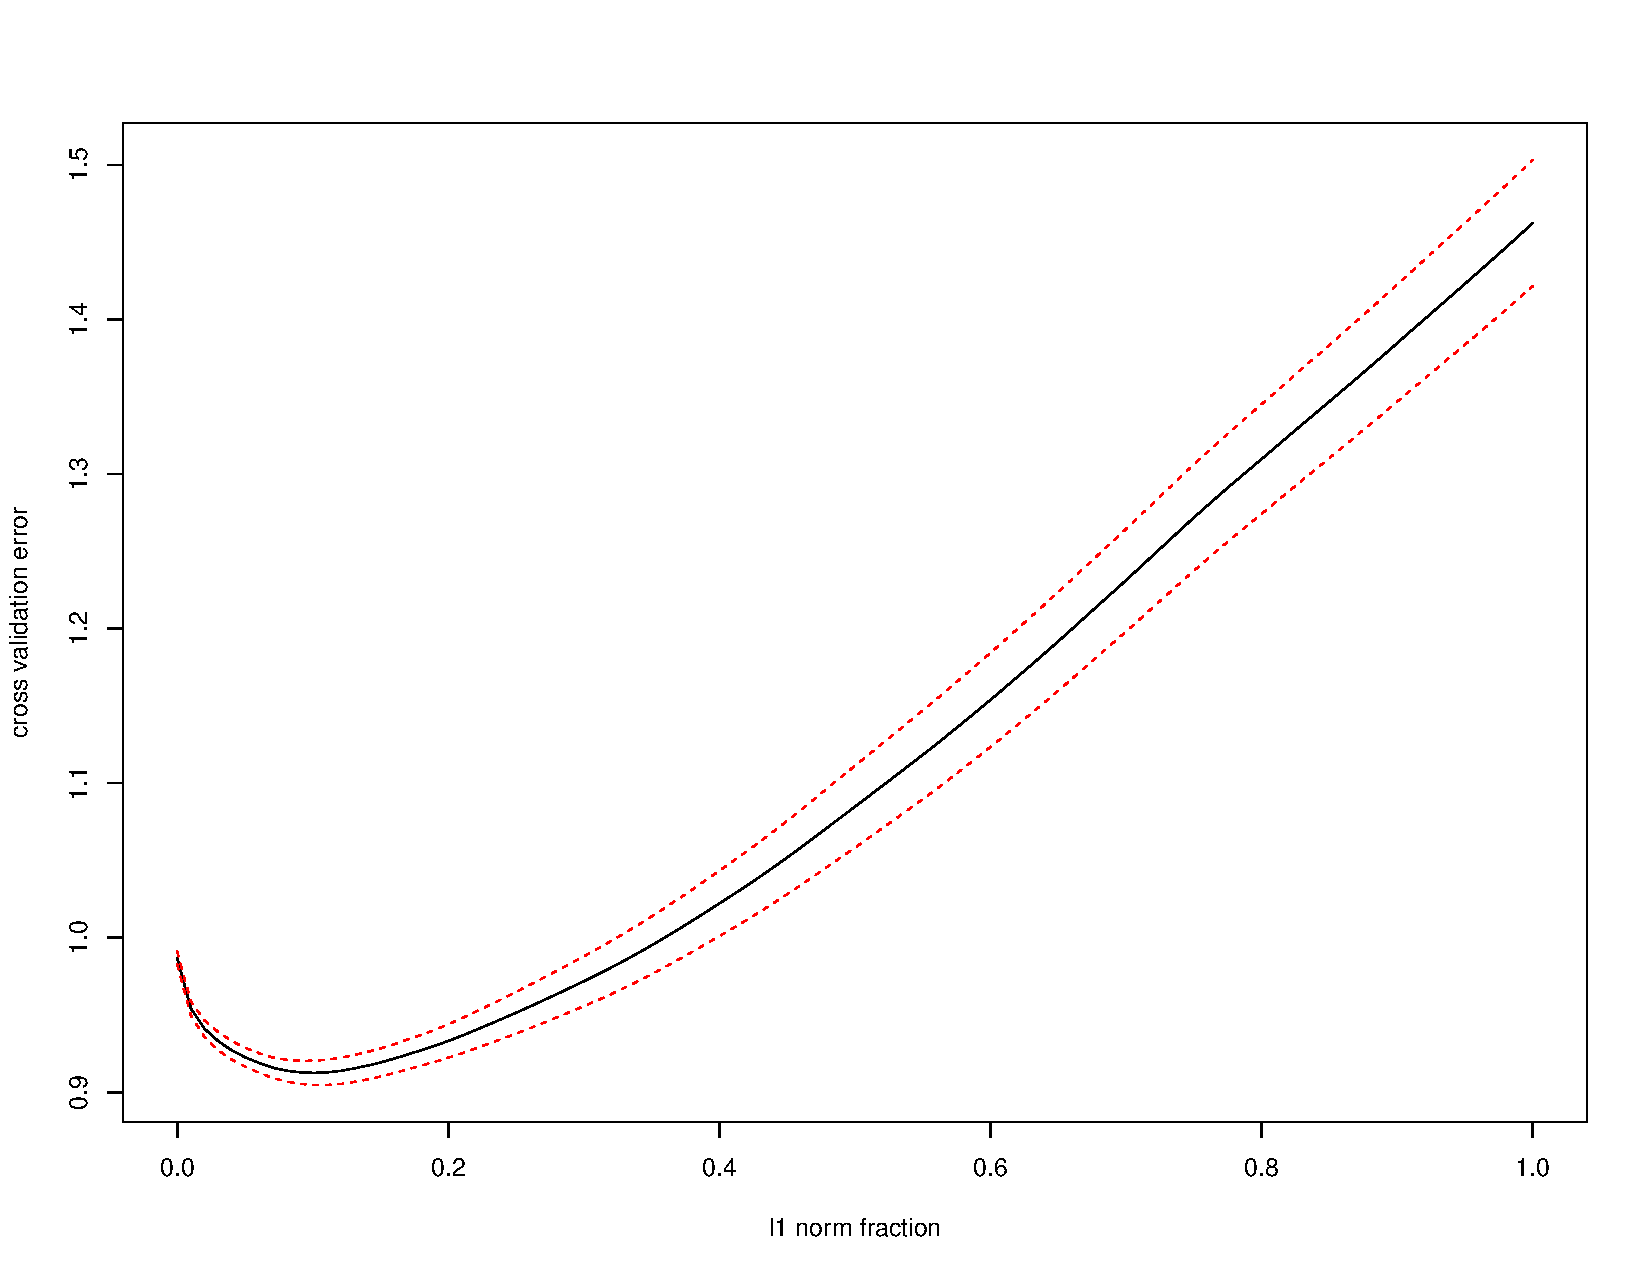
\includegraphics[height=0.9\textheight]{./../../lassoResults/CVNeuErr.pdf} 
%%\end{figure}
%%
%%\end{frame}
%%
%%%%%%%%%%%%%%%%%
%%\begin{frame}{LASSO: Spam}
%%
%%\begin{figure}
%%  \centering
%%  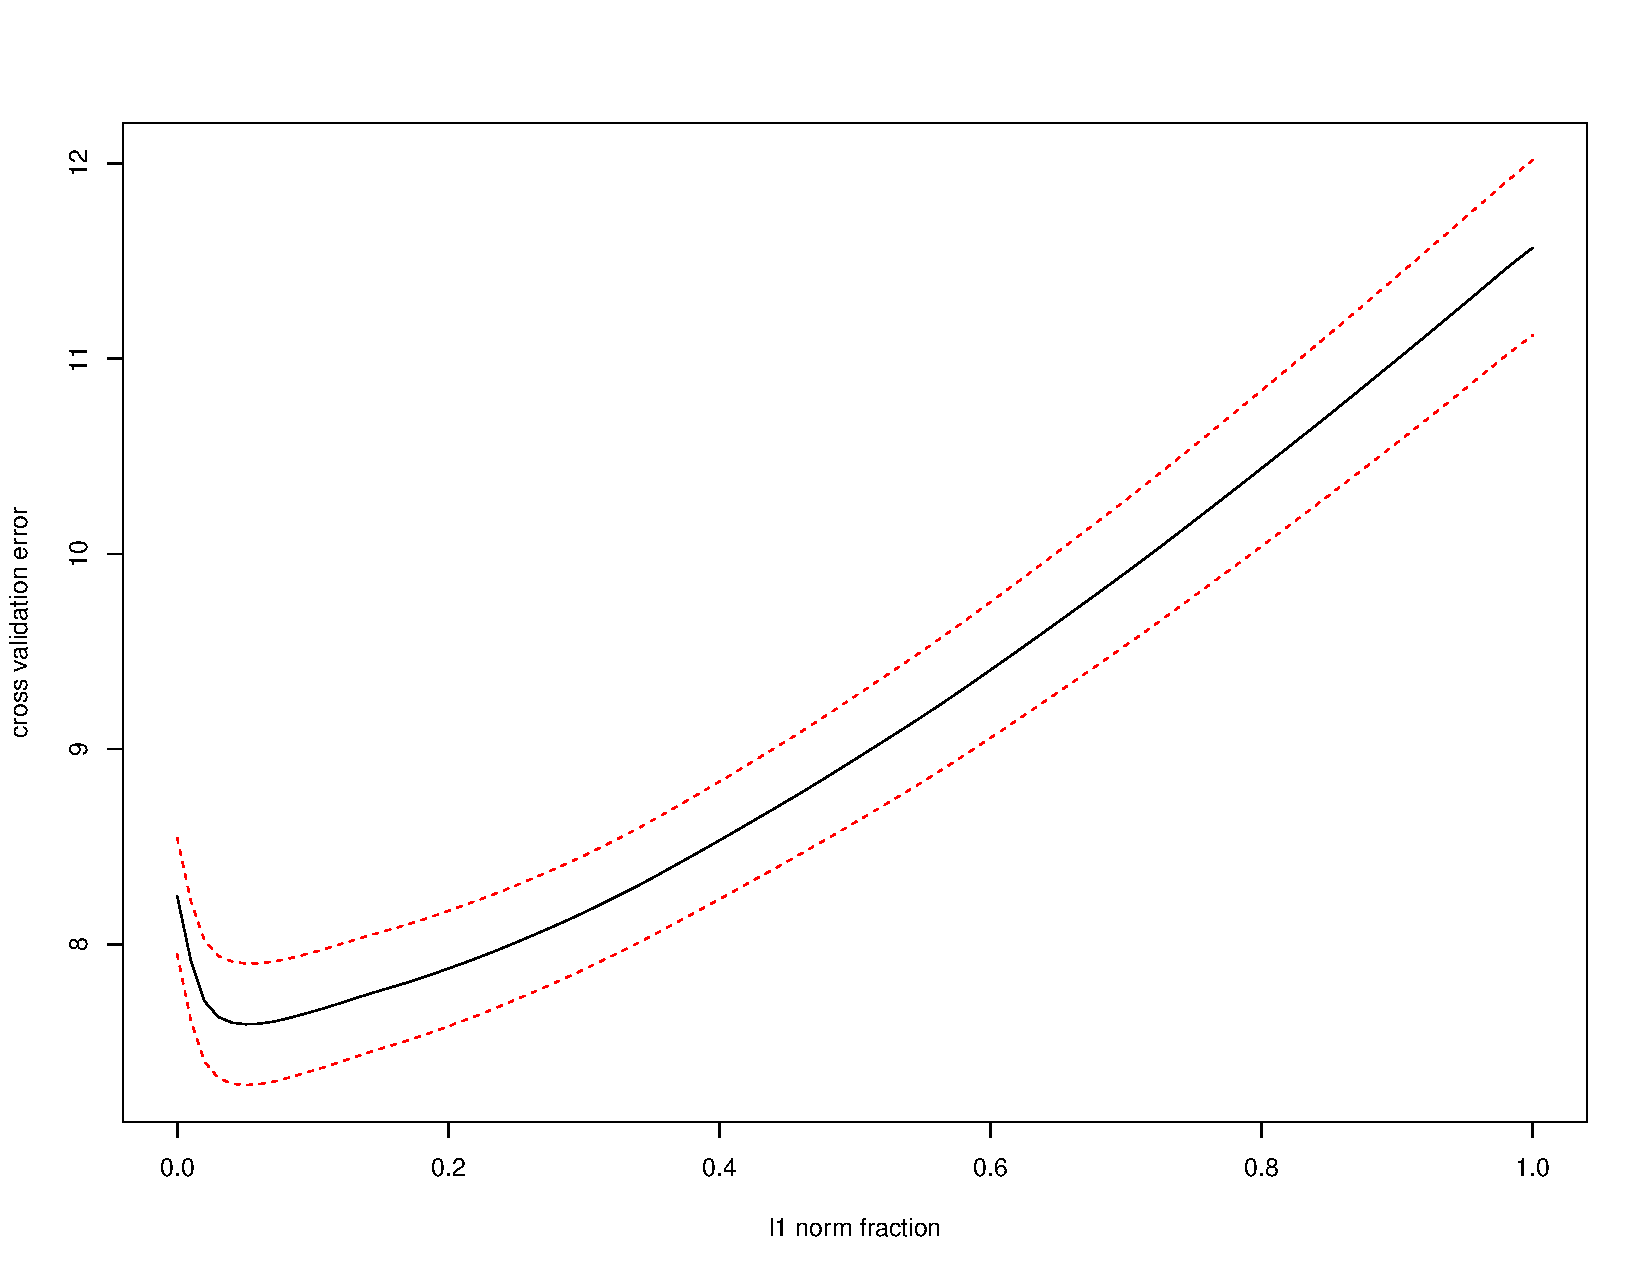
\includegraphics[height=0.9\textheight]{./../../lassoResults/CVSpamErr.pdf} 
%%\end{figure}
%%
%%\end{frame}
%%
%%%%%%%%%%%%%%%%

\subsection{$l_1$-Norm Support Vector Machine}
%%%%%%%%%%%%%%%
\begin{frame}[fragile]{Standard support vector machine}

\begin{itemize}[<+->]
\item Again, linear decision function $f(x) = \beta_0 + \beta x$;
\item The classifier $Class(x) = \textbf{sign} (f(x))$. 
\item  The support vector machine (SVM) (see, e.g. Hastie et al 2001): 
\begin{align*}
\min_{\beta_0,\beta} \sum_{i=1}^n(1-y_if(x_i))_+ + \frac{\lambda}{2} ||\beta||_2,
\end{align*}
where $z_+ = \max(0,z)$. 
\end{itemize}

\end{frame}


%%%%%%%%%%%%%%%
\begin{frame}[fragile]{$l_1$-Norm Support Vector Machine}

\begin{itemize}[<+->]  
\item Replacing the $l_2$-norm by $l_1$-norm yields the sparse SVM (Zhu et al 2003):
\begin{align*}
\min_{\beta_0,\beta} \left\{ \sum_{i=1}^n(1-y_i(\beta_0+\beta^Tx_i))_+ + \lambda ||\beta||_1\right\}. 
\end{align*}
\end{itemize}

\end{frame}


%%%%%%%%%%%%%%%%%%%%%%%%%%%%%%
%%%%%%%%%%%%%%%
\begin{frame}{Positive v.s. Nonpositive classification result}

\begin{itemize}[<+->]
\item +1: positive opinion;
\item -1: non-positive opinion, including negative, neutral and spam.
\item Cross validation result: 
  \begin{itemize}[<+->]
  \item training sample misclassification rate: 16.9\%
  \item testing sample misclassification rate: 28.2\%
  \end{itemize}

\end{itemize}


% put the table here

\end{frame}

%%%%%%%%%%%%%%%%%%%%%%%%
%%%%%%%%%%%%%%%
\begin{frame}{Negative v.s. Nonnegative classification result}
\begin{itemize}[<+->]
\item +1: negative opinion;
\item -1: non-negative opinion, including positive, neutral and spam.
\item Cross validation result: 
  \begin{itemize}[<+->]
  \item training sample misclassification rate: 6.4\%
  \item testing sample misclassification rate: 11.5\%
  \end{itemize}

\end{itemize}

%put the table here
\end{frame}

%%%%%%%%%%%%%%%
\begin{frame}{LASSO v.s. $l_1$-norm SVM}


\end{frame}

%%%%%%%%%%%%%%%%%%%%%%%%%%%%%%
\section{Further Work}

%%%%%%%%%%%%%%%
\begin{frame}{Further Work}

\begin{itemize}[<+->]
\item .
\end{itemize}

\end{frame}





%%%%%%%%%%%%%%%%%%%%%%%%%%%%%%
%%%%%%%%%%%%%%%%%%%%%%%%%%%%%%
%%%%%%%%%%%%%%%
\begin{frame}{}

\begin{itemize}[<+->]
\item  .
\end{itemize}

\end{frame}

%%%%%%%%%%%%%%%
\begin{frame}{}

\begin{itemize}[<+->]
\item  .
\end{itemize}

\end{frame}


%%%%%%%%%%%%%%%
\begin{frame}{}

\begin{itemize}[<+->]
\item  .
\end{itemize}

\end{frame}

%%%%%%%%%%%%%%%
\begin{frame}{}

\begin{itemize}[<+->]
\item .
\end{itemize}

\end{frame}


%%%%%%%%%%%%%%%
\begin{frame}{}

\begin{itemize}[<+->]
\item  .
\end{itemize}

\end{frame}

%%%%%%%%%%%%%%%
\begin{frame}{}

\begin{itemize}[<+->]
\item  .
\end{itemize}

\end{frame}

%%%%%%%%%%%%%%%
\begin{frame}{}

\begin{itemize}[<+->]
\item .
\end{itemize}

\end{frame}






\end{document}
